\documentclass[12pt,letterpaper]{article}
\usepackage[utf8]{inputenx} %Codificacion del texto (ISO Latin1 encoding)

\usepackage{fancyhdr} %Permite acomodar a tu gusto la parte de arriba y
% abajo del documento
\usepackage[spanish]{babel} %Permite definir el idioma del dcumento
\usepackage{graphicx} %Permite exportar imagenes en formato eps
\usepackage{url} %Tipo de fuente para correos y paginas
\usepackage{pgf}
\usepackage{fleqn}
\usepackage{amssymb}
\usepackage{amsmath}
\usepackage{fancyvrb}
\usepackage{makeidx}
\usepackage{colortbl} %Permite colocar colores a las tablas
\usepackage{multirow}
\usepackage{booktabs}
\usepackage{moreverb}
\usepackage{rotating}
\usepackage[final]{pdfpages}
%%%%%%%%%%
%Margenes%
%%%%%%%%%%
\parskip 1mm %Espacio entre parrafos

\setlength{\topmargin}{0pt}
\topmargin      0.5cm
\oddsidemargin	0.1cm  % Ancho Letter 21,59cm
\evensidemargin 0.5cm  % Alto  Letter 27,81cm
\textwidth	17cm%15.5cm
\textheight	21.0cm
\headsep	4 mm
\parindent	0.5cm
%%%%%%%%%%%%%%%%%%%%%%
%Estilo del documento%
%%%%%%%%%%%%%%%%%%%%%%
\pagestyle{fancyplain}

%%%%%%%%%%%%%%%%%%%%%%%%%%%%%%%%%%%%%%%%%%%
%Fancyheadings. Top y Bottom del documento%
%%%%%%%%%%%%%%%%%%%%%%%%%%%%%%%%%%%%%%%%%%%
% Recuerde que en este documento la portada del documento no posee
% numeracion, pero de igual manera llamaremos a esa primera pagina la numero
% 1, y la que viene la dos. Esto es para tener una idea de las que
% llamaremos pares e impares
\lhead{Computación Científica II} %Parte superior izquierda
\rhead{\bf \it Laboratorio 3} %Parte superior derecha
\lfoot{\it } %Parte inferior izquierda. \thepage indica
% el numero de pagina
\cfoot{} %Parte inferior central
\rfoot{\bf \thepage} %Parte inferior derecha
\renewcommand{\footrulewidth}{0.4pt} %Linea de separacion inferior

\newcommand{\primaria}[1]{
	\textbf{\underline{#1}}
}

\newcommand{\foranea}[1]{
	\textbf{\textsl{#1}}
}

\newcommand{\primyfor}[1]{
	\underline{\foranea{#1}}
}

\makeatletter
\newcommand\subsubsubsection{\@startsection {paragraph}{1}{\z@}%
                                   {-3.5ex \@plus -1ex \@minus -.2ex}%
                                   {1.5ex \@plus.2ex}%
                                   {\normalfont\bfseries}}
\newcommand\subsubsubsubsection{\@startsection {subparagraph}{1}{\z@}%
                                   {-3.5ex \@plus -1ex \@minus -.2ex}%
                                   {1.5ex \@plus.2ex}%
                                   {\normalfont\bfseries}}


\makeatother
 

\begin{document}
\title{Computación Científica II \\ \begin{Large}Laboratorio 3\end{Large}} 
\author{Victor Gonzalez Rodriguez\\victor.gonzalezro@alumnos.usm.cl\\2773029-9}
\date{\today}
\maketitle

\section{Introducción}
El cómputo de funciones complejas, o de las cuales no se tiene certeza de su naturaleza, puede ser un completo dolor de cabeza para científicos o estudiantes de ingeniería. Para una máquina, esto no pasa a ser algo más sencillo, es por esto, y para facilitar la vida de todos, es que existen algoritmos que facilitan el cálculo.

Podemos recurrir a la computación científica para resolver ecuaciones diferenciales también, utilizando distintos métodos, tales como el del disparo y realizando aproximaciones mediante métodos como el forward difference o backward difference.

En este laboratorio abarcaremos el cálculo de ecuaciones diferenciales calculadas mediante el método de backward difference.

\section{Objetivos}
\begin{itemize}
\item Implementar en Octave/Matlab la aproximación de forward difference.
\item Investigar sobre el método forward difference.
\item Comprobar las hipótesis y sus resultados.
\item Analizar resultados.
\end{itemize}

\section{Preguntas}
En esta sección se esbozará parte del enunciado original para dar un contexto. Toda información vaga respecto al enunciado se puede aclarar revisando el documento de los enunciados del laboratorio.

\subsection{eqHeatFD.m}
Se nos pide implementar en código Octave/Matlab el método forward difference de aproximación a la función de calor. Además se nos entregan las condiciones de borde y los parámetros del ejercicio.

El código que resuelve este problema es el siguiente:
\begin{verbatimtab}[4]
	for i = 1:MAX_ITER,
		u_j = A*u_prev';		
		u_j2 = u_j';
	
		u_j(1) = 0;
		u_j(m) = 0;
	
		local_dif = u_j' - u_prev;
		result(:,i) = u_prev;
		u_prev = u_j2;		
	
		% si nos aproximamos lo suficiente nos detenemos
		if max(abs(local_dif)) <= (1.1*10^(-4))
			result(:,i) = u_prev;
			break
		end
	end
\end{verbatimtab}

Donde A es la matriz tridiagonal definida por el método forward difference. Básicamente este el nucleo del método, ya que matemáticamente realizamos $u^{(i)} = A*u^{(i-1)}$, es decir, vamos iterando y vamos mejorando la aproximación al valor real de la solución de la ecuación diferencial del calor.

Esto se detiene bajo 2 condiciones: cuando $|u^{(i)} - u^{(i-1)}| \leq 1.1 * 10^{-4}$, o cuando se supere el máximo de iteraciones, que en este caso es $5000$.

El resultado de este programa entrega una aproximación a las soluciones del problema en los puntos que están al interior de los bordes de la malla generada.

\subsection{surfaceDataTime.m}
Se nos pide graficar el comportamiento de la función $u$, obtenido en el ejercicio anterior. El resultado es el siguiente:

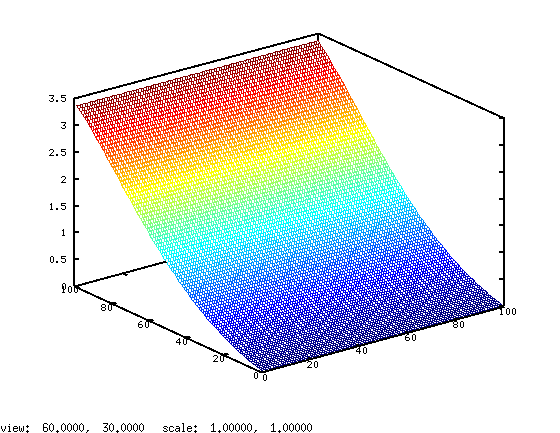
\includegraphics[width=\textwidth]{./pregunta2.png}
\\

Por favor notar que las iteraciones fueron \textbf{solo} 100, ya que de lo contrario la máquina de pruebas no entregaba imágen.

\subsection{surfaceDataInterval.m}
Se nos pide que, basados en el ejercicio 1, grafiquemos el comportamiento de la función $u$, a lo largo de un tiempo $t=20[s]$, para cada punto $x_i$, dentro de la porción de la barra en el intervalo $[0;0.5][m]$.

El resultado es el siguiente:

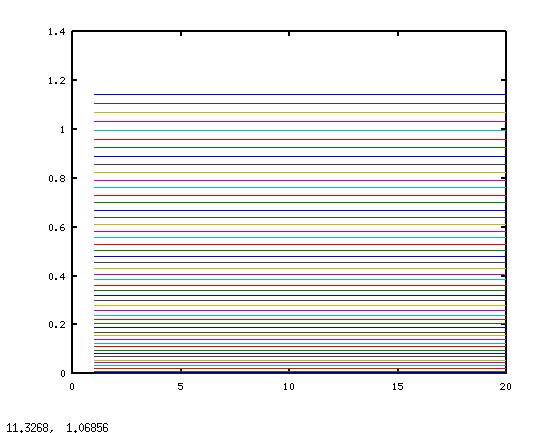
\includegraphics[width=\textwidth]{./pregunta3.png}
\section{Conclusiones}
Podemos concluir que mediante métodos algorítmicos y gracias a la computación moderna, podemos simplificar el cálculo de data compleja, mediante métodos numéricos. En nuestro caso, los métodos de aproximación de forward difference, nos ayudan a encontrar una buena aproximación de la solución a la ecuación diferencial del calor.
\newpage
\section{Anexos}
\subsection{Pregunta 1}
\begin{verbatim} 
octave:1> [res ans] = eqHeatFD(1,0.01,0.000000001,1,5000)
ans =  1
res = ... % matriz gigante
\end{verbatim}
\subsection{Pregunta 2}
\verb+octave:1> surfaceDataTime(1,0.01,0.000000001,1,100);+

\textit{Por favor comprender que mi máquina no es tan rápida, y por sobre las 300 iteraciones las imagenes no aparecían.}
\subsection{Pregunta 3}
\verb+octave:1> surfaceDataInterval(0.5,0.01,0.000000001,1,20);+
+
\end{document} 